\documentclass[12pt]{article}
\usepackage[utf8]{inputenc}
\usepackage{parskip}
\usepackage{markdown}
\usepackage{hyperref}
\usepackage{listings}
\usepackage{color}
\usepackage[subtle]{savetrees}
\usepackage{verbatim}
\usepackage{blindtext}
\usepackage{graphicx}

\title{\vspace{-2cm} \textbf{Session 2 - Let's Do Some Maths!} \\ UCAS Program 2020}

\author{Chloe Lau}
\date{August 2020}

\begin{document}
\setlength{\parindent}{4ex}
\setlength{\parskip}{1em}

\maketitle

\section{Why Maths?}
Computer Science is half a Maths degree, it basically is a subset of Maths.

So you might ask: what sort of maths do you do at university?

\begin{center}
    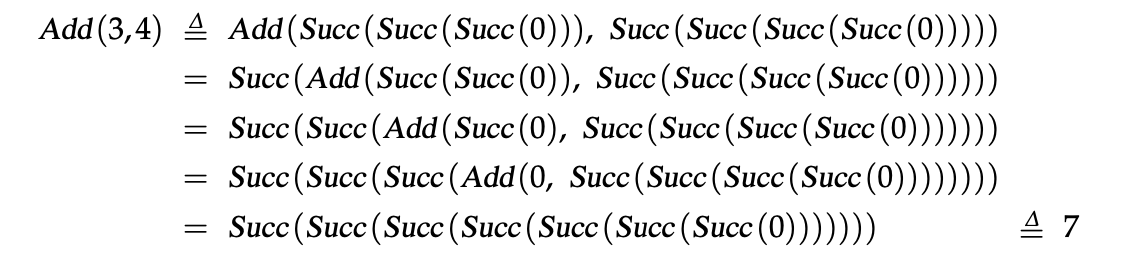
\includegraphics[scale=0.55]{add.png}
    A typical lemma in Discrete Maths.
\end{center}

Okay that is a joke that our lecturer included, but it still makes logical sense.

\begin{center}
    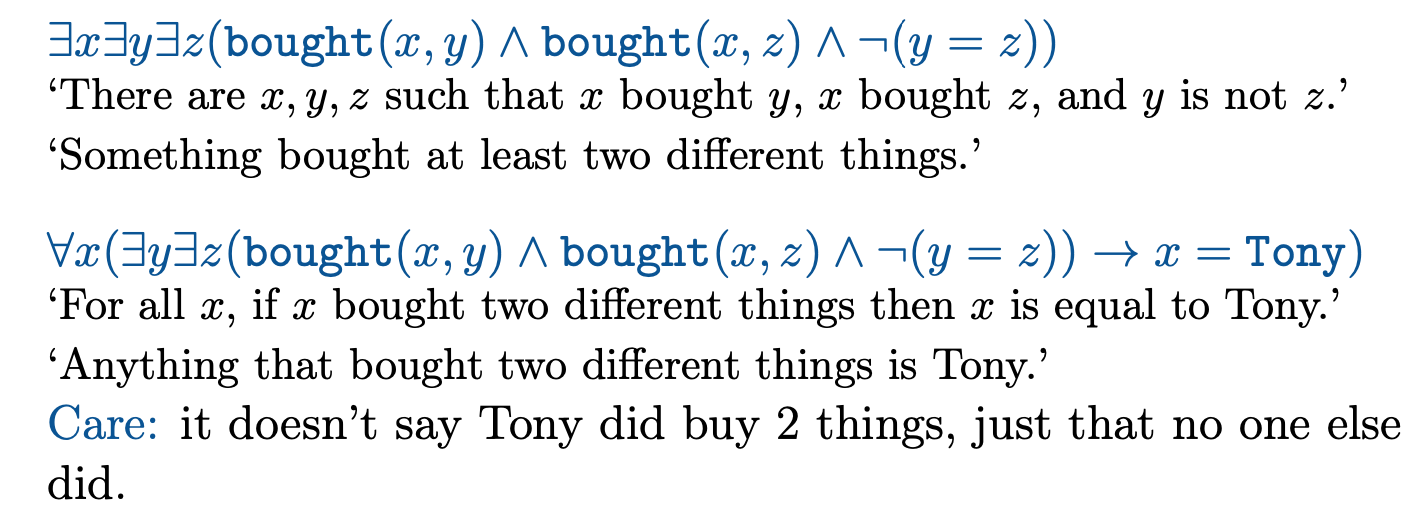
\includegraphics[scale=0.4]{logic.png}
    A snippet of my Logic Lecture Slides
\end{center}

Yes, sometimes we have to do translations to English too!

They are all Maths!

\section{The Real Maths at This Stage}
Applying to Computer Science, you have to prepare for \textbf{a lot of} admission tests:
\begin{itemize}
    \item CSAT - Cambridge
    \item TMUA - Cambridge and maybe Warwick
    \item MAT - Oxford and Imperial Maths
    \item STEP - Imperial \textbf{Computing or JMC} (almost guaranteed!), Imperial Maths, Cambridge Maths and CS)
\end{itemize}

Being mathy is a feature of a good Computer Scientist, but as a good Computer Scientist, being mathy isn't they only feature you need to carry.

What do you think is the most important to a Mathematician or Computer Scientist? Why do you think so?

What are your strongest parts in Mathematics? What do you find the most interesting in Mathematics? Theory? Statistics? Mechanics? Discrete?

How much maths have you done up till now? How confident are you with solving the questions?

How do you tackle these problems in an admission test? How would you tackle them in an interview otherwise?

Let's try some questions:

\subsection{MAT 2010, Q5}

\begin{center}
    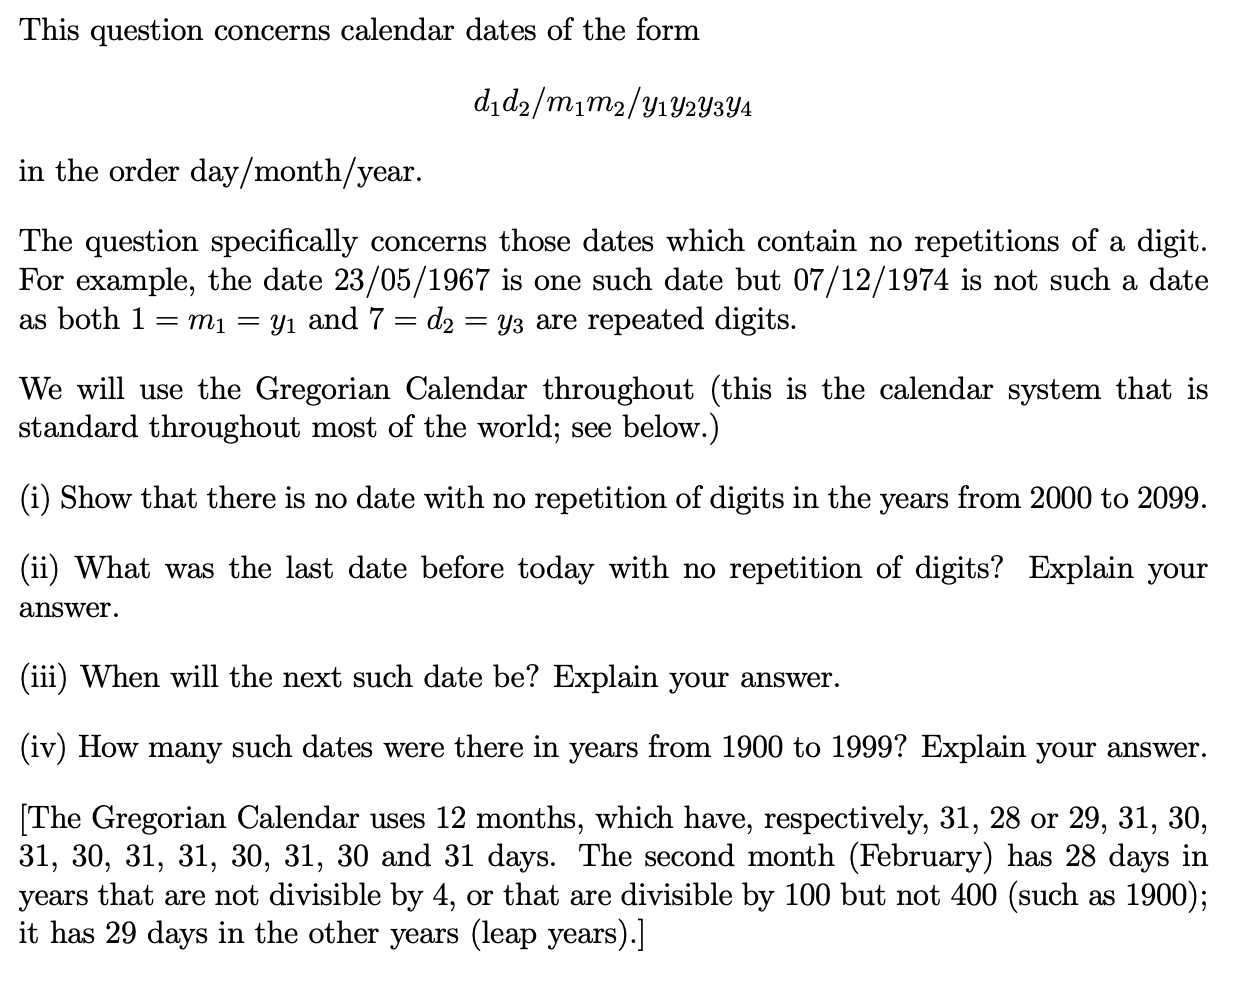
\includegraphics[scale=0.62]{date.png}
\end{center}

Some space for scribbles:

\subsection{STEP 2016, Paper 1, Q7}

\begin{center}
    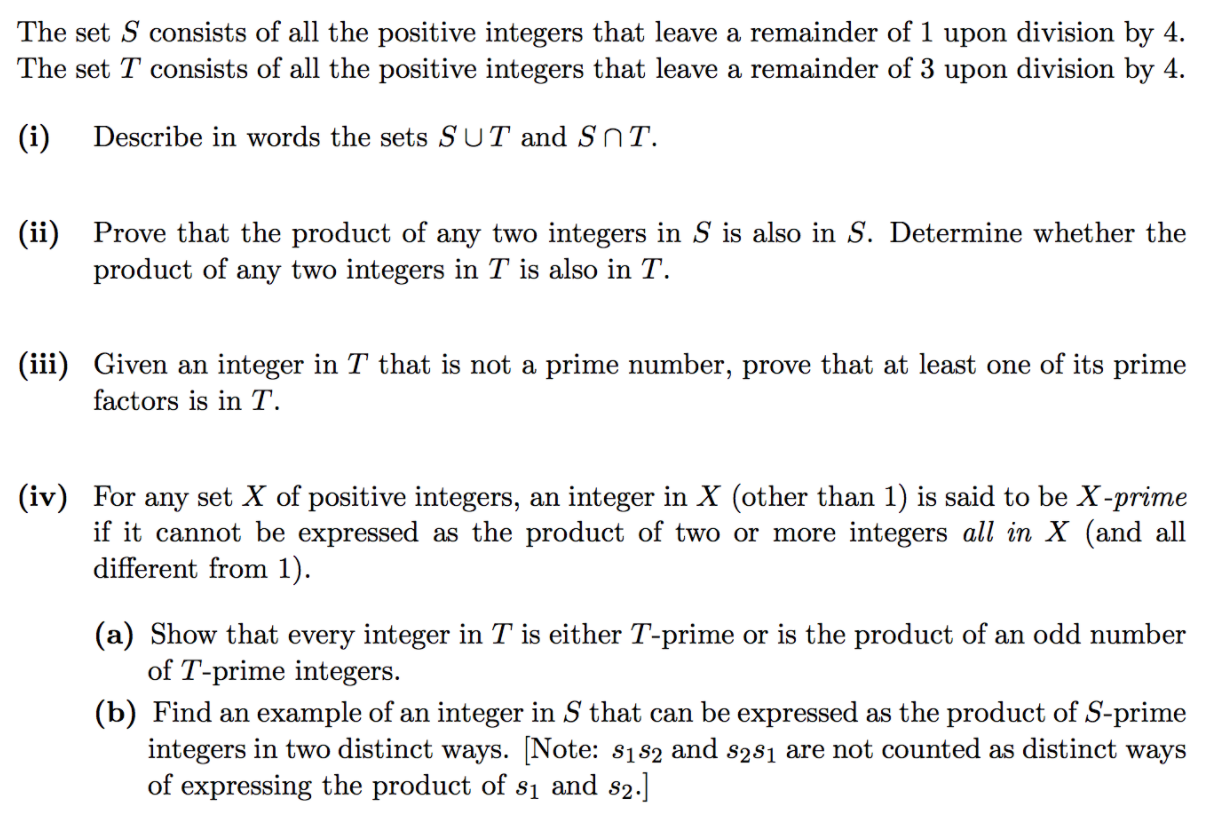
\includegraphics[scale=0.63]{settheory.png}
\end{center}

Some space for scribbles:

\end{document}
